\subsection{Pollution Ontology}

The Pollution ontology is extended from the  Pollution ODP as shown in Figure~\ref{fig:pollution-module}. The ODP has been adapted to the air pollution domain by extending some of the classes. For example, the \texttt{Pollutant} class is extended to \texttt{PrimaryPollutant} and \texttt{SecondaryPollutant}. \texttt{SecondaryPollutant} is further extended to \texttt{GaseousPol\-lutant} and \texttt{ParticulateMatter}. The sensors, observations, samples and actuator (SOSA) ontology includes concepts related to sensors and their observations. We derived \texttt{Contributor} from \href{http://www.w3.org/ns/sosa/FeatureOfInterest}{sosa:FeatureOfInterest}. With this, we can describe sensor observations with time and spatial information. The \href{https://www.w3.org/2003/01/geo/wgs84_pos#}{WGS84} vocabulary provides \href{http://www.w3.org/2003/01/geo/wgs84_pos#SpatialThing}{SpatialThing} for describing a spatial location on Earth. Figures~\ref{fig:reused-concepts-wgs84-sosa}, \ref{fig:air_pollution_concepts}, and \ref{fig:contributor_concepts} capture these re-used concepts in SAQI ontology. Some important concepts and properties from the Pollution module are discussed here.

\begin{figure}[ht]
\centering
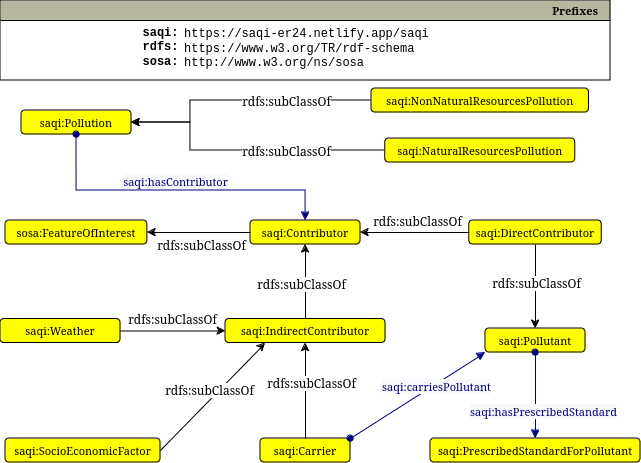
\includegraphics[height=6.8cm]{figures/ODP_subset_new.png}
\caption{Main concepts and properties of the Pollution module} 
\label{fig:pollution-module}
\end{figure}

%The sensors, observations, samples and actuator (SOSA) ontology includes concepts related to sensors and their observations. We derived \texttt{Contributor} from \href{http://www.w3.org/ns/sosa/FeatureOfInterest}{sosa:FeatureOfInterest}. With this, we can describe sensor observations with time and spatial information. The \href{https://www.w3.org/2003/01/geo/wgs84_pos#}{WGS84} vocabulary provides \href{http://www.w3.org/2003/01/geo/wgs84_pos#SpatialThing}{SpatialThing} for describing a spatial location on Earth. Figures~\ref{fig:reused-concepts-wgs84-sosa}, \ref{fig:air_pollution_concepts}, and \ref{fig:contributor_concepts} capture these re-used concepts in SAQI ontology. %We have also resused \href{http://xmlns.com/foaf/0.1/#term_Agent}{foaf:Agent} and schema TODO - ODPS, shcema, foaf etc.
 
\begin{figure}[ht]
\centering
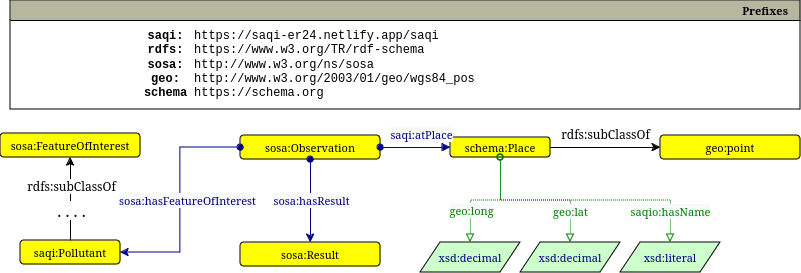
\includegraphics[height=3cm]{figures/reuse_new.png}
\caption{Re-used concepts from WGS84 and SOSA} 
\label{fig:reused-concepts-wgs84-sosa}
\end{figure}


\textbf{AirPollution.} This class is extended from the \texttt{Pollution} class of the Pollution ODP. The \texttt{Pollution} class represents the different types of contaminants in the natural environment. \texttt{AirPollution} is linked to \texttt{Pollutant} through the  \texttt{hasContributor} property (Axiom 1). The institutions working to mitigate the pollution sources through policies and awareness campaigns are linked by the object property \texttt{takesActionAgainst}. These properties and their connection with the \texttt{AirPollution} class are shown in Figure~\ref{fig:air_pollution_concepts}.

\begin{equation}
    \texttt{Pollution} \sqsubseteq \exists\texttt{hasContributor}.\texttt{Contributor}    
\end{equation}

\begin{figure}[ht]
\centering
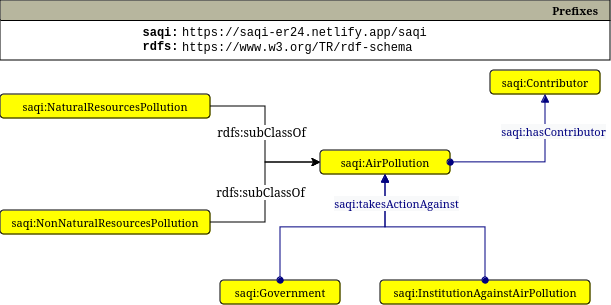
\includegraphics[height=4.5cm]{figures/airpoll_new.png}
\caption{AirPollution class and its connections} 
\label{fig:air_pollution_concepts}
\end{figure}

\textbf{hasContributor.} This object property connects the \texttt{AirPollution} class to its direct and indirect contributors (pollutants). %represent Direct or Indirect contributors that cause a particular kind of Pollution. In SAQI context, only, all contributors are linked to AirPollution instance of pollution.

\textbf{takesActionAgainst.} The institutions that are working to mitigate the effects of air pollution are connected through this object property. We considered two possible types of institutions -- government and non-government institutions such as NGOs. %that actively work on either reducing the pollutants causing Pollution, or reduce exposure to pollution in their geographical area of focus.

\textbf{Contributor.} It is a subclass of \href{http://www.w3.org/ns/sosa/FeatureOfInterest}{sosa:FeatureOfInterest},  allowing us to record observations of the contributors. A contributor can either be a contaminant particle, i.e., \texttt{Pollutant} or it could be a \texttt{Carrier} that transports a \texttt{Pollutant}. The \texttt{Contributor} class and other related classes are shown in Figure~\ref{fig:contributor_concepts}.

\begin{figure}[ht]
\centering
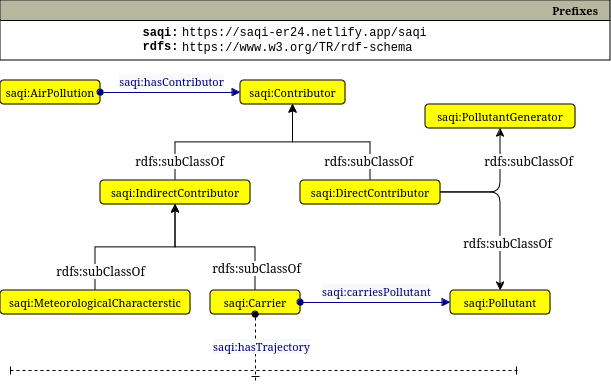
\includegraphics[height=6cm, width=0.80\textwidth]{figures/contrib_new.png}
\caption{Contributor class and its connections} 
\label{fig:contributor_concepts}
\end{figure}

\textbf{carriesPollutant.} This object property is used with an  \texttt{IndirectContributor} that transports a \texttt{Pollutant} from one spatial location to another, for example, wind and water flow.

\textbf{DirectContributor.} This class represents the contributors that directly impact pollution. \texttt{Pollutant} is a subclass of \texttt{Direct\-Contributor}. Some examples of pollutants include biological pollutants (viruses, pathogens, bacteria, etc.), chemical pollutants (toxic metal, radionuclides, organophosphorus compounds, gases, etc.) and physical pollutants (sound, thermal energy, space debris, etc.) present in the environment. 

\textbf{IndirectContributor.} This represents the things that indirectly contribute to pollution at a particular spatiotemporal point. These include environmental factors like temperature, the air or water streams flowing into or out of a particular place, the socio-economic factors such as policies and demographics. We have modelled only the \texttt{Carrier} concept as the subclass of \texttt{IndirectContributor} since other indirect contributors are specific to certain kinds of pollution.

\textbf{Carrier.} This concept is a subclass of the \texttt{IndirectContributor} concept and represents the air, water, and other kinds of streams flowing into or out of a particular place. It is linked to the \texttt{Trajectory} concept through the \texttt{hasTrajectory} property. Carriers are generally observed to affect the concentration of pollutants at a particular place and are important in modelling pollutants. To represent the pollutants that might be carried through a trajectory, the \texttt{Carrier} concept is linked to the \texttt{Pollutant} concept by the \texttt{carriesPollutant} property. %To specify the location of the source of pollutants in a carrier trajectory, \texttt{nearby} property can be used. This links the pollutant sources such as factories in the case of wind stream carrier or drains in the case of water stream carrier to the \texttt{TrajectoryPoint}. The applications that have such a requirement can make use of the \texttt{nearby} property, but we excluded it from the ODP because it is not sufficiently general.


\textbf{Pollutant.} \texttt{Pollutant} is a central concept in the Pollution module. It is  associated with the \texttt{Observation} class to keep a record of pollutant concentrations at any location and timestamp. Each pollutant has a prescribed standard that is defined by the government authorities. The \texttt{Pollutant} class and its connections are shown in Figure~\ref{fig:pollutant_concepts}. %The carrier concept can be used to track the flow of pollutants through location and time.

%\textbf{carriesPollutant.} Links an \texttt{IndirectContributor} which transports a \texttt{Pollutant} from one spatial location to another, for example, wind and water flow.

\textbf{hasPrescribedStandard.} Links a pollutant with standard limits based on concentration/amount of that pollutant in the environment. For example, WHO prescribed standard for PM$_{2.5}$ is less than 5 $\mu g/m^3$ mean concentration in the air annually. 

\textbf{hasObservation.} This is used to capture the concentration of a particular pollutant at a given time and spatial location.
    %\footnote{2005 WHO guidelines prescribe the  range for air pollutants such as particulate matter (PM), ozone ($O_3$), nitrogen dioxide ($NO_2$), etc., available at  \href{http://whqlibdoc.who.int/hq/2006/WHO\_SDE\_PHE\_OEH\_06.02\_eng.pdf}{http://whqlibdoc.who.int/hq/2006/WHO\_SDE\_PHE\_OEH\_06.02\_eng.pdf}}

\begin{figure}[ht]
\centering
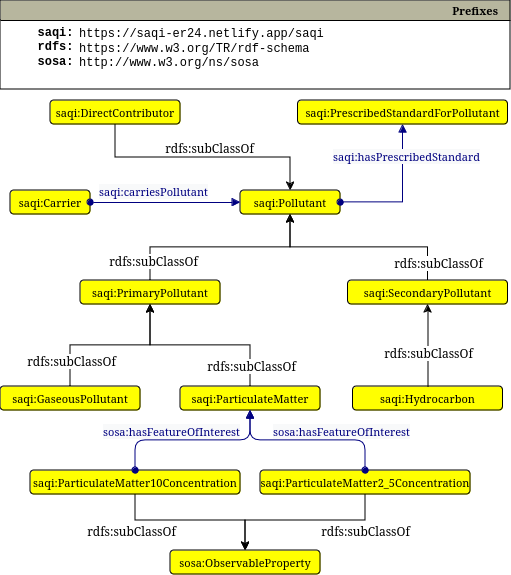
\includegraphics[height=8cm]{figures/pollutants_new.png}
\caption{Pollutant class and its connections} 
\label{fig:pollutant_concepts}
\end{figure}
    
\textbf{PrescribedStandardForPollutants.} This is a stub meta-pattern~\cite{stub_MP} that can be used to describe the prescribed ranges for pollutants. For a particular location, pollutants have a defined range of permissible concentrations that are specified by various global authorities. A standard for a pollutant may change with time and place. Hence the \texttt{PrescribedStandardFor\-Pollutant} concept is linked to the \texttt{Observation} concept by the \texttt{has\-Observation} property.

\textbf{PollutantGenerator.} Pollutant generators are events that generate pollution, such as crop burning, power plants, waste burning and dusty weather. It is related to the \texttt{Perception} class in the \emph{Ethnography} module, indicating the  perception of people on the severity of pollution concentration in a specific area. The \texttt{PollutantGenerator} class and its connections are shown in Figure~\ref{fig:pollutant_generator}.

\textbf{nearby.} This property links a pollution generator to a carrier trajectory.

\textbf{sourceResponsibleForLocalPollution.} The perception of pollution is directly linked to observable pollution generators in a locality, resulting in the perception of pollution by the people in that locality.


\begin{figure}[ht]
\centering
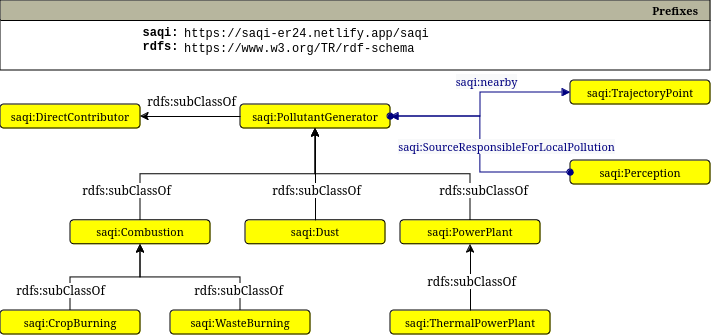
\includegraphics[height=6cm]{figures/pollutant_generator_new.png}
\caption{PollutantGenerator class and its connections} 
\label{fig:pollutant_generator}
\end{figure}

